\documentclass[11pt]{article}
\usepackage[T1]{fontenc}
\usepackage{lmodern}
\usepackage[margin=1in]{geometry}
\usepackage{amsmath,amssymb,amsthm}
\usepackage{microtype}
\usepackage{flafter}
\usepackage{enumitem}
\usepackage{tikz}
\usetikzlibrary{arrows.meta,positioning}
\usepackage[colorlinks=true,linkcolor=blue!45!black,citecolor=blue!45!black,urlcolor=blue!45!black]{hyperref}
\hypersetup{pdftitle={A superquadratic separation between sensitivity and block sensitivity}}
\newcommand{\bs}{\operatorname{bs}}
\newcommand{\unverified}[1]{\par\smallskip\noindent\fbox{\parbox{0.95\linewidth}{\textbf{Unverified step.} #1}}\par\smallskip}
\newtheorem{theorem}{Theorem}[section]
\newtheorem{lemma}[theorem]{Lemma}
\newtheorem{proposition}[theorem]{Proposition}
\newtheorem{corollary}[theorem]{Corollary}
\theoremstyle{definition}
\newtheorem{definition}[theorem]{Definition}
\newtheorem{example}[theorem]{Example}
\theoremstyle{remark}
\newtheorem{remark}[theorem]{Remark}
\title{A superquadratic separation between sensitivity\\and block sensitivity}
\author{Rewritten for readability from the OpenAI manuscript of the same title}
\date{}
\begin{document}
\maketitle
\begin{abstract}
We disprove the quadratic strengthening of the Sensitivity Conjecture by
constructing nonconstant total Boolean functions whose block sensitivity grows
faster than any constant multiple of sensitivity squared. In fact, for some
fixed \(\alpha>2\), our examples have unbounded block sensitivity and satisfy
\(\bs(f)\ge s(f)^\alpha\).
\end{abstract}

\section{Statement, context, and plan}
\label{sec:introduction}

\subsection{Definitions and results}

For a positive integer \(n\), write \([n]=\{1,\ldots,n\}\).
For \(x\in\{0,1\}^n\) and \(W\subseteq[n]\), let \(x^W\) be the string obtained from \(x\) by flipping exactly the coordinates in \(W\); write \(x^e\) for \(x^{\{e\}}\).
A \emph{total Boolean function} is any map \(f:\{0,1\}^n\to\{0,1\}\).
Its \emph{sensitivity} is
\[
 s(f,x)=\bigl|\{e\in[n]:f(x^e)\ne f(x)\}\bigr|,
 \qquad s(f)=\max_x s(f,x).
\]
A set \(W\subseteq[n]\) is a \emph{sensitive block for \(f\) at \(x\)} if \(f(x^W)\ne f(x)\).
The \emph{block sensitivity} \(\bs(f,x)\) is the largest number of pairwise disjoint nonempty sensitive blocks for \(f\) at \(x\), and \(\bs(f)=\max_x\bs(f,x)\).

\begin{theorem}\label{thm:main}
For every real \(C>0\), there are a positive integer \(n\) and a
nonconstant total Boolean function \(f:\{0,1\}^n\to\{0,1\}\) such that
\[
 \bs(f)>C\,s(f)^2.
\]
More precisely, for every integer \(d\ge1\) the construction below gives
a nonconstant total Boolean function \(f\) with
\[
 \frac{\bs(f)}{s(f)^2}\ge \frac{2^d}{4(d+2)^2}.
\]
\end{theorem}

\begin{corollary}
\label{cor:power-separation}
There exist a real number $\alpha>2$ and nonconstant total Boolean
functions $F_m$, for integers $m\geq1$, such that
\[
 \bs(F_m,0)\geq s(F_m)^\alpha
 \qquad\text{for every }m,
 \qquad
 \bs(F_m,0)\longrightarrow\infty.
\]
\end{corollary}

Theorem~\ref{thm:main} is proved in Section~\ref{sec:separation} and Corollary~\ref{cor:power-separation} in Section~\ref{sec:composition}.

\subsection{Context}

The Sensitivity Conjecture asked whether block sensitivity is bounded by a
polynomial in sensitivity, uniformly over the number of inputs and the
function. The question goes back to Nisan's work on parallel computation,
which introduced block sensitivity and already recorded Rubinstein's
quadratic separation \cite[Section~2]{Nisan1989}.
Nisan and Szegedy studied the problem through the degree of the unique
multilinear real polynomial representing a Boolean function, and explicitly
suggested the quadratic inequality \(\bs(f)\le s(f)^2\)
\cite[Section~4]{NisanSzegedy1994}.
Rubinstein's construction \cite{Rubinstein1995} showed that a polynomial
upper bound would need degree at least two. Virza improved the separation
to \(\bs(f)=\tfrac12s(f)^2+\tfrac12s(f)\) \cite{Virza2011}, and
Ambainis and Sun obtained examples with
\(\bs(f)=\frac23s(f)^2-\frac13s(f)\)
\cite[Theorem~1]{AmbainisSun2011}.
These improvements left open whether any universal quadratic upper bound
could hold.
Huang resolved the polynomial conjecture in 2019. His degree bound,
together with Tal's refinement of the degree--block-sensitivity comparison
\cite{Tal2013}, gives \(\bs(f)\le s(f)^4\) for every total Boolean function
\cite[Theorem~1.5]{Huang2019}. Wellens later improved the leading constant,
proving \(\bs(f)\le\sqrt{2/3}\,s(f)^4+1\)
\cite[Corollary~4.2]{Wellens2022}.
Theorem~\ref{thm:main} rules out the quadratic strengthening.

\paragraph{Relation to earlier constructions.}
Meiburg's spectral-sensitivity construction uses tournament-indexed rows
of positive conditions and one selected blocking coordinate in each
outgoing row \cite[Sections~3.1 and~5.2--5.5]{Meiburg2026}.\footnote{In the
attribution accompanying this construction, Meiburg credits GPT-5.6-Sol
with the gated-tournament ideas and describes his own contributions as
exposition, size and parameter optimization, and checking the faithfulness
of the Lean formalization.}
There, random labels exclude small local configurations in which many accepting
subcubes lie close to the same accepting input. The present paper adapts this architecture
to nested predicates, using a different forbidden-label condition and a
direct union bound.
The sensitivity graph joins adjacent cube inputs exactly when the function
changes value. Its maximum degree is \(s(f)\); spectral sensitivity
\(\lambda(f)\) is the operator norm of its adjacency matrix
\cite{AaronsonEtAl2021}.
Since \(\lambda(f)\le s(f)\), a lower bound on
\(\bs(f)/\lambda(f)^2\) alone does not supply the ordinary-sensitivity
separation in Theorem~\ref{thm:main}; the estimates below are proved directly, without a spectral input.
The final OR of disjoint copies follows the balancing principle of Ambainis and Sun
\cite[Section~4, Lemma~1]{AmbainisSun2011}.
Ambainis and Pr\={u}sis explicitly
noted that a seed with block sensitivity greater than sensitivity squared
would yield a superquadratic power separation by iteration
\cite[Section~1]{AmbainisPrusis2014}. Composition as an amplification method
is treated systematically by Tal~\cite{Tal2013}; the two composition facts needed here are proved in Lemma~\ref{lem:composition}.

\subsection{Proof at a glance}
\label{sec:glance}

Fix \(d\ge1\) and a large integer \(M\) (eventually \(M\ge9^{d+1}\)), and put \(L=d+2\), \(k=2M^2+1\), \(r=\lceil\sqrt M\rceil\).

\paragraph{The objects.}
For each \emph{level} \(\ell=0,\ldots,d\) we define \(d+1-\ell\) predicates
\(P_{\ell,1}\ge P_{\ell,2}\ge\cdots\ge P_{\ell,d+1-\ell}\) on the same input space (a larger index is a stronger predicate).
Level \(0\) consists of indicators of unions of Hamming balls of radii \(d,d-1,\ldots,0\) around \(M\) far-apart centres.
A level-\(\ell\) input is a \(k\times r\) array of level-\((\ell-1)\) inputs (``children'').
The rows are the vertices of a fixed tournament in which every row beats \(M^2\) others.
The predicate \(P_{\ell,q}\) accepts if for some row \(i\) the following \emph{clause} holds: the strongest level-\((\ell-1)\) predicate accepts all \(r\) children of row \(i\) (\emph{targets}), and for every row \(j\) beaten by \(i\), a weaker level-\((\ell-1)\) predicate rejects one designated child of row \(j\) (\emph{gates}).
The designated child is given by an edge label \(a(i,j)\in[r]\); the index \(q\) selects which weaker predicate the gates use.

\paragraph{The two quantities.}
At the all-zero input every predicate is \(0\), and there are \(Mk^\ell\) disjoint blocks whose flip makes it \(1\) (Lemma~\ref{lem:blocks}); the number of blocks is multiplied by \(k>2M^2\) per level.
Let \(S_{\ell,0}\) and \(S_{\ell,1}\) be the largest sensitivities of level-\(\ell\) predicates at \(0\)-inputs and at \(1\)-inputs.
The aim is \(S_{\ell,b}\le2LM^{\ell+b}\) (Lemma~\ref{lem:quantitative-profiles}): each sensitivity is multiplied by about \(M\) per level, so its square grows by \(M^2\) while the block count grows by \(k\ge2M^2\).
This gains a factor \(2\) per level.

\paragraph{Why sensitivity grows only by a factor \(M\).}
\begin{itemize}[leftmargin=*]
\item \emph{At a \(1\)-input} a flip must break one fixed satisfied clause, which has \(M^2\) gates and \(r\) targets. This gives \(S_{\ell,1}\le M^2S_{\ell-1,0}+rS_{\ell-1,1}\approx M^2S_{\ell-1,0}\).
\item \emph{At a \(0\)-input} a flip must complete a clause that is exactly one condition short. Clauses one \emph{target} short number at most \(15\); this is what the edge labels are chosen for (Lemma~\ref{lem:labelling}). Clauses one \emph{gate} short number at most \(3\), by a counting argument in the tournament. For all but one of them, the failed gate sits on a child that the strongest predicate accepts, so repairing the gate forces \emph{two} distinct predicates of that child to flip simultaneously.
\item This is why we also track \emph{joint} sensitivities \(J_{\ell,b}\): the largest number of single-bit flips that change two fixed distinct predicates of level \(\ell\) at once. They are \(0\) at level \(0\), because one bit changes a Hamming distance by \(1\) and cannot cross two integer radii. They stay negligible when \(M\) is large. The result is \(S_{\ell,0}\le16S_{\ell-1,0}+S_{\ell-1,1}+3J_{\ell-1,1}\approx S_{\ell-1,1}\).
\end{itemize}

\paragraph{Steps and dependencies.}
\begin{enumerate}[leftmargin=*]
\item Lemma~\ref{lem:labelling}: a good edge labelling exists (probabilistic method). Used only in Step~C3 of Proposition~\ref{prop:recurrences}.
\item Lemma~\ref{lem:clauses}: each clause uses distinct children, and the predicates are nested. Used throughout Proposition~\ref{prop:recurrences}.
\item Lemma~\ref{lem:base}: sensitivity bounds at level \(0\). This starts the induction in Lemma~\ref{lem:quantitative-profiles}.
\item Lemma~\ref{lem:blocks}: disjoint sensitive blocks at zero. Used for the lower bound on \(\bs\) in Theorem~\ref{thm:main}.
\item Proposition~\ref{prop:recurrences}: four recurrences for \(S_{\ell,b},J_{\ell,b}\). This is the core of the paper.
\item Lemma~\ref{lem:quantitative-profiles}: solving the recurrences gives \(S_{\ell,b}\le2LM^{\ell+b}\) when \(M\ge9^{d+1}\).
\item Theorem~\ref{thm:main}: take the OR of \(M\) disjoint copies of the single top-level predicate \(P_{d,1}\). This multiplies the \(0\)-side sensitivity and the block count by \(M\) and leaves the \(1\)-side sensitivity unchanged, balancing the two sides at \(2LM^{d+1}\).
\item Lemma~\ref{lem:composition} and the case \(d=9\) of Step~7 give Corollary~\ref{cor:power-separation} by iterated composition.
\end{enumerate}

\begin{center}
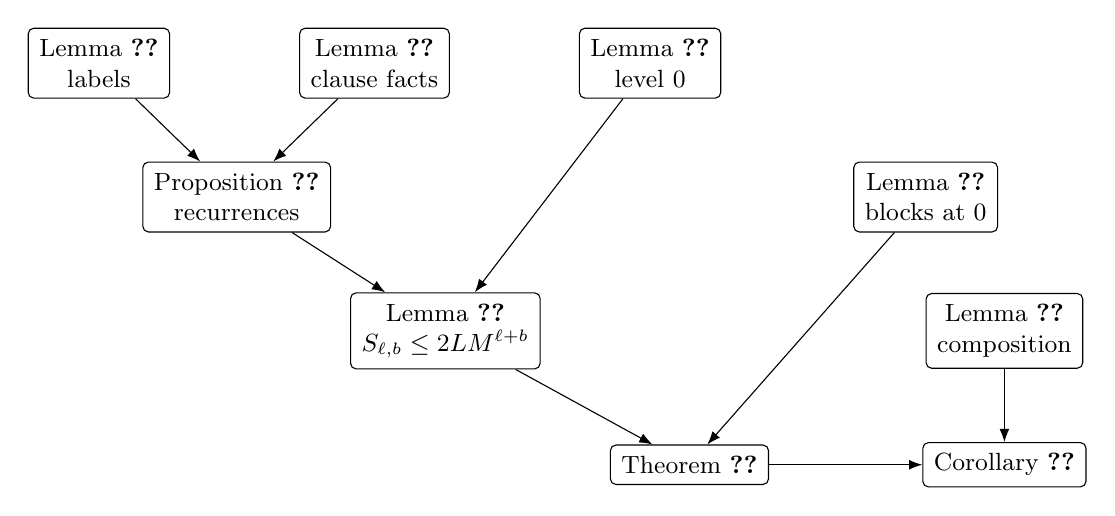
\begin{tikzpicture}[>=Latex, every node/.style={font=\small},
  box/.style={draw,rounded corners=2pt,inner sep=4pt,align=center}]
 \node[box] (lab) at (0,0) {Lemma~\ref{lem:labelling}\\labels};
 \node[box] (facts) at (3.5,0) {Lemma~\ref{lem:clauses}\\clause facts};
 \node[box] (base) at (7,0) {Lemma~\ref{lem:base}\\level \(0\)};
 \node[box] (rec) at (1.75,-1.7) {Proposition~\ref{prop:recurrences}\\recurrences};
 \node[box] (blocks) at (10.5,-1.7) {Lemma~\ref{lem:blocks}\\blocks at \(0\)};
 \node[box] (quant) at (4.4,-3.4) {Lemma~\ref{lem:quantitative-profiles}\\\(S_{\ell,b}\le2LM^{\ell+b}\)};
 \node[box] (comp) at (11.5,-3.4) {Lemma~\ref{lem:composition}\\composition};
 \node[box] (main) at (7.5,-5.1) {Theorem~\ref{thm:main}};
 \node[box] (cor) at (11.5,-5.1) {Corollary~\ref{cor:power-separation}};
 \draw[->] (lab) -- (rec);
 \draw[->] (facts) -- (rec);
 \draw[->] (rec) -- (quant);
 \draw[->] (base) -- (quant);
 \draw[->] (quant) -- (main);
 \draw[->] (blocks) -- (main);
 \draw[->] (main) -- (cor);
 \draw[->] (comp) -- (cor);
\end{tikzpicture}
\end{center}

\paragraph{Note to the reader.}
One sentence of the source proof (Step~B1 in the proof of Proposition~\ref{prop:recurrences}) applies the nesting of the predicates in the wrong direction. It is reproduced and flagged there.

\paragraph{Notation changes relative to the source.}
A flipped coordinate is called \(e\) (source: \(a\), which clashed with the labels \(a(i,j)\)).
Blocks are called \(W\) (source: \(B\)).
The size of the list \(\mathcal G\) is called \(\gamma\) (source: \(m\)).
In Lemma~\ref{lem:composition} the arities are \(n_f,n_g\), the block counts \(p_f,p_g\) and the blocks \(\Gamma_i,\Delta_j\) (source: \(a,b,p,q,C_i,D_j\)).

\section{The labelled tournament and nested predicates}
\label{sec:construction}

\subsection{Parameters}

Fix integers \(d\ge1\) and \(M\ge3\), and put
\[
 L=d+2,\qquad k=2M^2+1,\qquad r=\lceil\sqrt M\rceil,
 \qquad t=16.
\]
Until Section~\ref{sec:separation} only \(M\ge3\) is used; there \(M\ge9^{d+1}\) is imposed.
For \(0\le\ell\le d\), set
\[
 H_\ell=d+1-\ell,\qquad N_\ell=LM(kr)^\ell.
\]
Here \(H_\ell\) is the number of predicates at level \(\ell\) and \(N_\ell\) is their number of input bits.
Note \(H_{\ell-1}=H_\ell+1\) and \(H_d=1\).

\subsection{The tournament and its labelling}

A \emph{tournament} on a vertex set is an orientation of every pair of distinct vertices: exactly one of \(i\to j\) and \(j\to i\) holds.
We use a tournament on \([k]\) in which every vertex has outdegree \(M^2\).
One exists: place the \(k=2M^2+1\) vertices on a cycle and let \(i\to j\) when \(j\) is one of the next \(M^2\) vertices after \(i\).
For distinct \(i,j\), the cyclic distance from \(i\) to \(j\) lies in \(\{1,\ldots,2M^2\}\), and it is at most \(M^2\) exactly when the distance from \(j\) to \(i\) is not.
So exactly one orientation holds.

The tournament rows and selected blocking coordinates adapt the architecture
of Meiburg~\cite[Sections~3.1 and~5.2--5.5]{Meiburg2026}.
The label property needed here is the following.
It is used once, in Step~C3 of the proof of Proposition~\ref{prop:recurrences}.

\begin{lemma}\label{lem:labelling}
The edges can be labelled by numbers \(a(i,j)\in[r]\) so that there is
no set \(I\subseteq[k]\) of size \(t\) admitting choices
\(m_j\in[r]\), \(j\in I\), with
\[
 a(i,j)=m_j \qquad\text{for every edge }i\to j\text{ within }I.
\]
\end{lemma}
\begin{proof}
We use the probabilistic method with a union bound.
\begin{enumerate}[leftmargin=*]
\item Choose all edge labels independently and uniformly from \([r]\).
\item Fix a set \(I\) of size \(t=16\) and values \((m_j)_{j\in I}\). There are \(\binom{16}{2}=120\) edges within \(I\), one for each pair. For each such edge \(i\to j\) the event \(a(i,j)=m_j\) has probability \(1/r\). These events concern different edges, so they are independent. All of them hold with probability \(r^{-120}\).
\item There are at most \(k^{16}\) sets \(I\) and \(r^{16}\) tuples \((m_j)\). By the union bound, the probability that some pair \((I,(m_j))\) satisfies all its equalities is at most
\[
 k^{16}r^{16}r^{-120}=k^{16}r^{-104}\le (3M^2)^{16}(\sqrt M)^{-104}
 =3^{16}M^{32-52}=3^{16}M^{-20}\le3^{-4}<1.
\]
Here we used \(k=2M^2+1\le3M^2\), \(r\ge\sqrt M\), and \(M\ge3\).
\item Hence with positive probability no pair \((I,(m_j))\) satisfies all its equalities, so a labelling with the required property exists.\qedhere
\end{enumerate}
\end{proof}

Fix such a labelling for the remainder of the construction; we call it \emph{admissible}.

\subsection{Nested families}

We construct predicates \(P_{\ell,q}:\{0,1\}^{N_\ell}\to\{0,1\}\), for \(0\le\ell\le d\) and
\(1\le q\le H_\ell\), that are \emph{nested}:
\[
 P_{\ell,1}(x)\ge P_{\ell,2}(x)\ge\cdots
 \ge P_{\ell,H_\ell}(x)\quad\text{for every }x.
\]
Nesting concerns the predicate index, not the input bits.
We use it in the following two forms, for indices \(q<q'\):
\begin{itemize}[leftmargin=*]
\item[(N1)] if \(P_{\ell,q'}(x)=1\) then \(P_{\ell,q}(x)=1\);
\item[(N0)] if \(P_{\ell,q}(x)=0\) then \(P_{\ell,q'}(x)=0\).
\end{itemize}
So the predicate with the \emph{larger} index is the \emph{stronger} one (harder to satisfy).
Nesting is proved in Lemma~\ref{lem:clauses}(c).

\paragraph{Level \(0\).}
Partition \([LM]\) into \(M\) blocks \(E_1,\ldots,E_M\), each of
size \(L\). Let \(z_j\in\{0,1\}^{LM}\) be the string that is one precisely on \(E_j\) (the \(j\)-th \emph{centre}).
Write \(\operatorname{dist}\) for Hamming distance and set
\[
 D(x)=\min_{j\in[M]}\operatorname{dist}(x,z_j),\qquad
 P_{0,q}(x)=\mathbf1\{D(x)\le H_0-q\}\quad(1\le q\le H_0=d+1).
\]
The radii \(H_0-q\) are the integers from \(d\) (for \(q=1\)) down to \(0\) (for \(q=d+1\)).
Distinct centres have disjoint supports of size \(L\), so their distance is \(2L=2d+4\).

\paragraph{Level \(\ell\ge1\).}
Let \(1\le\ell\le d\). Split the \(N_\ell\) input bits into \(kr\) disjoint
\emph{children} \(x_{j,c}\in\{0,1\}^{N_{\ell-1}}\), arranged in \(k\) rows
\(j\in[k]\), each with \(r\) positions \(c\in[r]\).
For this level put
\[
 H=H_\ell,\qquad Q=H+1=H_{\ell-1}.
\]
For \(q\in[H]\) and a row \(i\in[k]\), \emph{clause \(i\) at index \(q\)} asserts
\begin{equation}\label{eq:predicate-definition}
 \begin{aligned}
 P_{\ell-1,Q}(x_{i,c})&=1 &&\text{for all }c\in[r] &&\text{(target conditions)},\\
 P_{\ell-1,Q-q}(x_{j,a(i,j)})&=0 &&\text{for all }j\text{ with }i\to j &&\text{(gate conditions)}.
 \end{aligned}
\end{equation}
Define \(P_{\ell,q}(x)=1\) if clause \(i\) at index \(q\) holds for at least one \(i\in[k]\), and \(P_{\ell,q}(x)=0\) otherwise.
Figure~\ref{fig:clause} depicts the target row and one outgoing gate.

\begin{figure}[htbp]
\centering
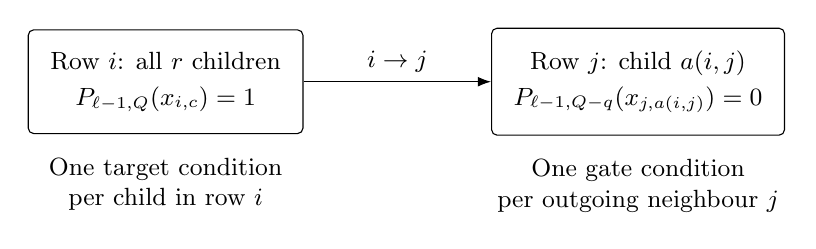
\begin{tikzpicture}[>=Latex, every node/.style={font=\small},
  condition/.style={draw,rounded corners=2pt,inner sep=8pt,align=center}]
 \node[condition] (target) at (0,0)
   {Row \(i\): all \(r\) children\\[2pt]
    \(P_{\ell-1,Q}(x_{i,c})=1\)};
 \node[condition] (gate) at (6,0)
   {Row \(j\): child \(a(i,j)\)\\[2pt]
    \(P_{\ell-1,Q-q}(x_{j,a(i,j)})=0\)};
 \draw[->] (target) -- node[above]{\(i\to j\)} (gate);
 \node[below=5pt of target,align=center] {One target condition\\per child in row \(i\)};
 \node[below=5pt of gate,align=center] {One gate condition\\per outgoing neighbour \(j\)};
\end{tikzpicture}
\caption{One recursive clause. The edge label selects a single child in
each outgoing neighbour's row. Raising \(q\) strengthens the gates;
all targets use the strongest child predicate \(Q\).}
\label{fig:clause}
\end{figure}

\begin{lemma}[Basic facts about clauses]\label{lem:clauses}
Let \(1\le\ell\le d\), \(H=H_\ell\), \(Q=H+1\).
\begin{enumerate}[label=\textup{(\alph*)},leftmargin=*]
\item For \(q\in[H]\) we have \(1\le Q-q\le H<Q\). So \(Q-q\) and \(Q\) are two distinct valid indices at level \(\ell-1\).
\item For fixed \(i\) and \(q\), the \(r+M^2\) conditions of clause \(i\) concern \(r+M^2\) distinct children. Consequently, flipping one input coordinate changes the truth value of at most one condition of clause \(i\), and only a condition on the child containing that coordinate.
\item If \(q<q'\) and clause \(i\) holds at \(x\) at index \(q'\), then clause \(i\) holds at \(x\) at index \(q\). Consequently the predicates \(P_{\ell,1},\ldots,P_{\ell,H}\) are nested. The level-\(0\) predicates are nested as well.
\item \(P_{\ell,q}\) is a total Boolean function on \(krN_{\ell-1}=N_\ell\) bits.
\end{enumerate}
\end{lemma}
\begin{proof}
(a) \(1\le q\le H\) gives \(Q-H\le Q-q\le Q-1\), that is, \(1\le Q-q\le H\).

(b) The targets use the children \((i,c)\), \(c\in[r]\), all in row \(i\). Each gate uses a child in a row \(j\ne i\), and distinct gates use distinct rows \(j\), because there is one edge between \(i\) and each other row. There are \(M^2\) gates since \(i\) has outdegree \(M^2\). Each coordinate lies in exactly one child, and the truth value of a condition depends only on its own child.

(c) We argue by induction on the level. At level \(0\), if \(q<q'\) then \(H_0-q'<H_0-q\), so \(D(x)\le H_0-q'\) implies \(D(x)\le H_0-q\); this is (N1). Now let \(\ell\ge1\) and assume level \(\ell-1\) is nested. The target conditions do not depend on the index. Let \(y=x_{j,a(i,j)}\) be a gate child. The gate at index \(q'\) says \(P_{\ell-1,Q-q'}(y)=0\). Since \(Q-q'<Q-q\), (N0) at level \(\ell-1\) gives \(P_{\ell-1,Q-q}(y)=0\), which is the gate at index \(q\). So clause \(i\) at index \(q'\) implies clause \(i\) at index \(q\). Therefore \(P_{\ell,q'}(x)=1\) implies \(P_{\ell,q}(x)=1\).

(d) There are \(kr\) children of \(N_{\ell-1}\) bits each, and \(kr\cdot LM(kr)^{\ell-1}=N_\ell\).
\end{proof}

\begin{example}[The case \(d=1\)]
Here \(L=3\), \(H_0=2\), \(H_1=1\). Level \(0\) has \(P_{0,1}=\mathbf 1\{D\le1\}\) and \(P_{0,2}=\mathbf 1\{D=0\}\) on \(3M\) bits.
Level \(1\) has the single predicate \(P_{1,1}\), with \(Q=2\) and \(Q-q=1\).
Clause \(i\) says that every child of row \(i\) equals some centre exactly, and that for each \(j\) with \(i\to j\) the child \(x_{j,a(i,j)}\) is at distance at least \(2\) from every centre.
\end{example}

\subsection{Sensitivity profiles and the initial bounds}

For \(b\in\{0,1\}\), define the \emph{ordinary profile}
\[
 S_{\ell,b}=\max_{\substack{1\le q\le H_\ell,\ x\in\{0,1\}^{N_\ell}\\
                           P_{\ell,q}(x)=b}}
 \bigl|\{e\in[N_\ell]:P_{\ell,q}(x^e)=1-b\}\bigr|
\]
and the \emph{joint profile}
\[
 J_{\ell,b}=\max_{\substack{1\le q<q'\le H_\ell,\ x\in\{0,1\}^{N_\ell}\\
                         P_{\ell,q}(x)=P_{\ell,q'}(x)=b}}
 \bigl|\{e\in[N_\ell]:P_{\ell,q}(x^e)=P_{\ell,q'}(x^e)=1-b\}\bigr|.
\]
A maximum over no cases is defined to be zero; in particular
\(J_{d,0}=J_{d,1}=0\), since \(H_d=1\).
In \(J_{\ell,b}\) the two predicates are evaluated on the same input and changed by the same bit.
In Section~\ref{sec:recurrences} the definitions are used in the following form, for a level-\(\ell\) input \(y\):
\begin{itemize}[leftmargin=*]
\item[(CS)] if \(P_{\ell,g}(y)=b\), then at most \(S_{\ell,b}\) coordinates \(e\) satisfy \(P_{\ell,g}(y^e)=1-b\);
\item[(CJ)] if \(g\ne g'\) and \(P_{\ell,g}(y)=P_{\ell,g'}(y)=b\), then at most \(J_{\ell,b}\) coordinates \(e\) satisfy \(P_{\ell,g}(y^e)=P_{\ell,g'}(y^e)=1-b\).
\end{itemize}

The next lemma starts the induction in Lemma~\ref{lem:quantitative-profiles}.

\begin{lemma}\label{lem:base}
The initial sensitivity profiles satisfy
\begin{equation}\label{eq:base-profile}
 S_{0,0}\le L,\qquad S_{0,1}\le LM,\qquad
 J_{0,0}=J_{0,1}=0.
\end{equation}
\end{lemma}
\begin{proof}
\emph{Step 1: \(|D(x^e)-D(x)|\le1\).}
For every centre \(z_j\), \(\operatorname{dist}(x^e,z_j)=\operatorname{dist}(x,z_j)\pm1\).
Taking \(j\) with \(\operatorname{dist}(x,z_j)=D(x)\) gives \(D(x^e)\le D(x)+1\). The same argument with \(x\) and \(x^e\) exchanged gives \(D(x)\le D(x^e)+1\).

\emph{Step 2: \(J_{0,0}=J_{0,1}=0\).}
Let \(q<q'\), with radii \(R=H_0-q\) and \(R'=H_0-q'\). These are integers with \(R\ge R'+1\).
If both predicates are \(0\) at \(x\) and both are \(1\) at \(x^e\), then \(D(x)\ge R+1\) and \(D(x^e)\le R'\), so \(D(x)-D(x^e)\ge R+1-R'\ge2\).
If both are \(1\) at \(x\) and both are \(0\) at \(x^e\), then \(D(x)\le R'\) and \(D(x^e)\ge R+1\), so \(D(x^e)-D(x)\ge2\).
Both cases contradict Step~1, so no such \(e\) exists.

\emph{Step 3: \(S_{0,0}\le L\).}
Fix \(q\), put \(R=H_0-q\in\{0,\ldots,d\}\), and let \(D(x)\ge R+1\) (that is, \(P_{0,q}(x)=0\)).
Suppose \(P_{0,q}(x^e)=1\). Then some centre \(z_j\) has \(\operatorname{dist}(x^e,z_j)\le R\), hence \(\operatorname{dist}(x,z_j)\le R+1\), hence \(\operatorname{dist}(x,z_j)=R+1\) because \(D(x)\ge R+1\).
At most one centre lies within distance \(d+1\) of \(x\): two such centres would be at distance at most \(2d+2<2d+4=2L\) from each other.
Since \(R+1\le d+1\), the centre \(z_j\) is the same for every successful \(e\).
Moreover \(\operatorname{dist}(x^e,z_j)=\operatorname{dist}(x,z_j)-1\), so \(e\) is one of the \(R+1\) coordinates where \(x\) and \(z_j\) differ.
There are thus at most \(R+1\le d+1\le L\) successful flips.

\emph{Step 4: \(S_{0,1}\le LM\).} This is the total number \(N_0=LM\) of input bits.
\end{proof}

\subsection{Disjoint blocks at zero}

The next lemma gives the lower bound on block sensitivity in the proof of Theorem~\ref{thm:main}.

\begin{lemma}\label{lem:blocks}
At every level \(0\le\ell\le d\), all predicates are zero at the
all-zero input. There are \(Mk^\ell\) pairwise disjoint nonempty blocks
of coordinates, each of size \(Lr^\ell\), such that flipping any one
block at zero makes every predicate at that level equal to one.
\end{lemma}
\begin{proof}
We use induction on \(\ell\).

\emph{Level \(0\).} Every centre has weight \(L\), so \(D(0)=L>d\), and all radii are at most \(d\). Hence all predicates vanish at \(0\).
The blocks \(E_1,\ldots,E_M\) are disjoint of size \(L\), and \(0^{E_j}=z_j\) has \(D(z_j)=0\), so every \(P_{0,q}(z_j)=1\).

\emph{Level \(\ell\ge1\), assuming the claim at level \(\ell-1\).}
\begin{enumerate}[leftmargin=*]
\item At the all-zero input every child is all-zero, so by induction every target \(P_{\ell-1,Q}(x_{i,c})\) equals \(0\). Every clause has \(r\ge1\) targets, so every clause fails and every \(P_{\ell,q}(0)=0\).
\item Let \(W_1,\ldots,W_{Mk^{\ell-1}}\subseteq[N_{\ell-1}]\) be the block family of level \(\ell-1\). For a row \(i\in[k]\) and an index \(h\), let \(W_{i,h}\) be the union of the copies of \(W_h\) in the \(r\) children of row \(i\). It has size \(r\cdot Lr^{\ell-1}=Lr^\ell\).
\item After flipping \(W_{i,h}\) at zero, each child of row \(i\) equals \(0^{W_h}\) and all other children are all-zero. By induction, every level-\((\ell-1)\) predicate is \(1\) on \(0^{W_h}\) and \(0\) on \(0\). So all targets of clause \(i\) hold. The gate children of clause \(i\) lie in rows \(j\ne i\), are all-zero, and so have \(P_{\ell-1,Q-q}=0\) for every \(q\). All gates hold. Thus clause \(i\) holds at every index \(q\), and every \(P_{\ell,q}\) equals \(1\).
\item The sets \(W_{i,h}\) and \(W_{i',h'}\) are disjoint if \(i\ne i'\) because they lie in different rows. They are disjoint if \(i=i'\) and \(h\ne h'\) because \(W_h\cap W_{h'}=\emptyset\) inside each child. There are \(k\cdot Mk^{\ell-1}=Mk^\ell\) of them.\qedhere
\end{enumerate}
\end{proof}

\section{Sensitivity recurrences}
\label{sec:recurrences}

The following estimates hold for every input, including
inputs far from the blocks used in Lemma~\ref{lem:blocks}.
They feed Lemma~\ref{lem:quantitative-profiles}.

\begin{proposition}\label{prop:recurrences}
For $1\leq \ell\leq d$, write
$S'_b=S_{\ell-1,b}$ and $J'_b=J_{\ell-1,b}$.  Then
\begin{equation}\label{eq:recurrences}
\begin{aligned}
 S_{\ell,1}&\leq M^2S'_0+rS'_1,
 &\qquad J_{\ell,1}&\leq M^2J'_0+rS'_1,\\
 S_{\ell,0}&\leq tS'_0+S'_1+3J'_1,
 &\qquad J_{\ell,0}&\leq tS'_0+3J'_1.
\end{aligned}
\end{equation}
\end{proposition}

\paragraph{Plan of the proof.}
All four inequalities follow one scheme.
Fix the parent input \(x\) and the index \(q\) (or the pair \(q<q'\)).
Identify a small set of clauses, determined before the flipped coordinate is chosen, such that every flip being counted must change one specific condition of one of these clauses.
Then bound the number of coordinates in the child of that condition that can make the required change, using (CS) or (CJ) at level \(\ell-1\).
Summing over children is a union bound: a coordinate may be counted for several clauses, which only weakens the bound.
Parts A and B treat parent value \(1\); Parts C and D treat parent value \(0\).

\begin{proof}
Fix $\ell$, put $H=H_\ell$ and $Q=H+1$, and recall
\eqref{eq:predicate-definition}: at parent index $q$, every
target tests $P_{\ell-1,Q}=1$ and every gate tests
$P_{\ell-1,Q-q}=0$ on its child.
All flips are flips of a single coordinate \(e\) of the level-\(\ell\) input. Such a flip changes exactly one child, and by Lemma~\ref{lem:clauses}(b) it changes at most one condition of any fixed clause.
We place no restriction on how many nested predicates of that child change.

\medskip\noindent\textbf{Part A: \(S_{\ell,1}\le M^2S'_0+rS'_1\).}
\begin{enumerate}[label=\textbf{A\arabic*.},leftmargin=*]
\item Fix \(q\) and \(x\) with \(P_{\ell,q}(x)=1\), and fix a clause \(i\) that holds at \(x\) at index \(q\).
\item If \(P_{\ell,q}(x^e)=0\), then clause \(i\) fails at \(x^e\). So \(e\) lies in one of the \(r+M^2\) children used by clause \(i\) and turns that child's condition from true to false.
\item If the child is a gate child, its predicate \(P_{\ell-1,Q-q}\) changes from \(0\) to \(1\). By (CS) at most \(S'_0\) coordinates of that child do this. There are \(M^2\) gate children.
\item If the child is a target child, its predicate \(P_{\ell-1,Q}\) changes from \(1\) to \(0\). By (CS) at most \(S'_1\) coordinates do this. There are \(r\) target children.
\item Summing gives at most \(M^2S'_0+rS'_1\) flips.
\end{enumerate}

\medskip\noindent\textbf{Part B: \(J_{\ell,1}\le M^2J'_0+rS'_1\).}
\begin{enumerate}[label=\textbf{B\arabic*.},leftmargin=*]
\item Fix \(q<q'\) and \(x\) with \(P_{\ell,q}(x)=P_{\ell,q'}(x)=1\). The source proceeds: ``Choose a clause initially satisfied for \(q\); nesting makes it satisfied for \(q'\) as well. This same clause is fixed for all flips being counted.''
\unverified{The nesting is applied in the wrong direction. By Lemma~\ref{lem:clauses}(c), for \(q<q'\) a clause that holds at index \(q'\) holds at index \(q\), not conversely: the gates at index \(q'\) require the weaker child predicate \(P_{\ell-1,Q-q'}\ge P_{\ell-1,Q-q}\) to vanish, so a clause can hold at \(q\) and fail at \(q'\). Steps B2--B4 use only that the fixed clause holds at \(x\) at \emph{both} indices. Such a clause exists if one instead picks a clause satisfied at index \(q'\) (possible since \(P_{\ell,q'}(x)=1\)) and applies Lemma~\ref{lem:clauses}(c). With that choice I believe the inequality for \(J_{\ell,1}\) is correct, but the sentence as written is not justified.}
From here on, \(i\) denotes a clause that holds at \(x\) at both indices \(q\) and \(q'\).
\item Let \(e\) be a flip with \(P_{\ell,q}(x^e)=P_{\ell,q'}(x^e)=0\). In particular clause \(i\) fails at \(x^e\) at index \(q\). Either (i) some target of clause \(i\) is false at \(x^e\), or (ii) all its targets are true at \(x^e\) and some gate of clause \(i\) at index \(q\) is false at \(x^e\).
\item Case (i): the target was true at \(x\), so \(e\) lies in that target child and changes \(P_{\ell-1,Q}\) from \(1\) to \(0\). By (CS) this accounts for at most \(S'_1\) coordinates per target child, hence at most \(rS'_1\) flips.
\item Case (ii): put
\[
 g=Q-q,\qquad g'=Q-q',\qquad 1\leq g'<g<Q.
\]
Let \(y\) be the child of the gate that fails at \(x^e\); the gate at index \(q\) held at \(x\), so \(e\) lies in \(y\).
Before the flip: clause \(i\) holds at index \(q'\), so \(P_{\ell-1,g'}(y)=0\), and (N0) gives \(P_{\ell-1,g}(y)=0\).
After the flip: the gate at index \(q\) fails, so \(P_{\ell-1,g}(y^e)=1\), and (N1) gives \(P_{\ell-1,g'}(y^e)=1\).
So the two distinct child predicates \(P_{\ell-1,g'}\) and \(P_{\ell-1,g}\) both change from \(0\) to \(1\). By (CJ) at most \(J'_0\) coordinates of \(y\) do this. With \(M^2\) gate children, case (ii) accounts for at most \(M^2J'_0\) flips.
\end{enumerate}
Adding B3 and B4 gives the bound.

\medskip\noindent\textbf{Part C: candidate clauses at a zero, and \(S_{\ell,0}\le tS'_0+S'_1+3J'_1\).}
\begin{enumerate}[label=\textbf{C\arabic*.},leftmargin=*]
\item Fix \(q\) and \(x\) with \(P_{\ell,q}(x)=0\). All clauses below are taken at index \(q\). Let \(\mathcal T\) be the set of clauses that at \(x\) fail exactly one target and no gate, and \(\mathcal G\) the set of clauses that at \(x\) fail exactly one gate and no target. These sets depend only on \(x\) and \(q\), not on any flip.
\item \emph{Every successful flip repairs a clause of \(\mathcal T\cup\mathcal G\).} Let \(P_{\ell,q}(x^e)=1\), and let clause \(i\) hold at \(x^e\). It fails at \(x\), and by Lemma~\ref{lem:clauses}(b) only one of its conditions differs between \(x\) and \(x^e\). So at \(x\) it has exactly one false condition, that is, \(i\in\mathcal T\cup\mathcal G\). Moreover \(e\) lies in the child of that condition and makes the condition true.
\item \emph{\(|\mathcal T|\le15<t\).} For \(j\in\mathcal T\), let \(m_j\in[r]\) be the position of its unique false target. Then \(P_{\ell-1,Q}(x_{j,m_j})=0\), and \(P_{\ell-1,Q}(x_{j,c})=1\) for \(c\ne m_j\). Let \(i,j\in\mathcal T\) with \(i\to j\), and put \(y=x_{j,a(i,j)}\). Clause \(i\) has no false gate, so \(P_{\ell-1,Q-q}(y)=0\). Since \(Q-q<Q\), (N0) at level \(\ell-1\) gives \(P_{\ell-1,Q}(y)=0\). So the target of row \(j\) at position \(a(i,j)\) is false, and uniqueness forces \(a(i,j)=m_j\). If \(|\mathcal T|\ge16\), any \(16\)-element subset \(I\subseteq\mathcal T\) with the values \((m_j)_{j\in I}\) would contradict Lemma~\ref{lem:labelling}.
\item \emph{Contribution of \(\mathcal T\).} A flip repairing clause \(j\in\mathcal T\) lies in the child \(x_{j,m_j}\) and changes \(P_{\ell-1,Q}\) there from \(0\) to \(1\). By (CS) there are at most \(S'_0\) such coordinates. With C3, \(\mathcal T\) accounts for at most \(15S'_0\le tS'_0\) flips.
\item \emph{Structure of \(\mathcal G\).} If \(j\in\mathcal G\), all targets of row \(j\) are true: \(P_{\ell-1,Q}(x_{j,c})=1\) for all \(c\). Let \(i,j\in\mathcal G\) with \(i\to j\), and put \(y=x_{j,a(i,j)}\). Then \(P_{\ell-1,Q}(y)=1\), and (N1) gives \(P_{\ell-1,Q-q}(y)=1\). So the gate of clause \(i\) in row \(j\) is false. Clause \(i\) has only one false gate, so \(i\) has at most one out-neighbour inside \(\mathcal G\). Let \(\gamma=|\mathcal G|\). The tournament induced on \(\mathcal G\) has \(\gamma(\gamma-1)/2\) edges and all outdegrees at most \(1\), so
\[
 \frac{\gamma(\gamma-1)}2\leq \gamma,
 \qquad\text{hence}\qquad \gamma\leq3.
\]
At most one vertex of \(\mathcal G\) has outdegree \(0\) inside \(\mathcal G\), since the edge between any two vertices leaves one of them.
\item \emph{A vertex \(i\in\mathcal G\) with an out-edge \(i\to j\) inside \(\mathcal G\).} By C5 the gate on \(y=x_{j,a(i,j)}\) is the unique false gate of clause \(i\), and \(P_{\ell-1,Q-q}(y)=P_{\ell-1,Q}(y)=1\). A flip \(e\) repairing clause \(i\) lies in \(y\) and gives \(P_{\ell-1,Q-q}(y^e)=0\), and then (N0) gives \(P_{\ell-1,Q}(y^e)=0\). The indices \(Q-q\) and \(Q\) are distinct because \(q\ge1\). By (CJ) at most \(J'_1\) coordinates repair clause \(i\). Such a flip also destroys a target of row \(j\), but that is irrelevant: we are only bounding the number of flips from above.
\item \emph{The possible vertex of \(\mathcal G\) with no out-edge inside \(\mathcal G\).} A flip repairing it changes \(P_{\ell-1,Q-q}\) from \(1\) to \(0\) on the child of its unique false gate. By (CS) there are at most \(S'_1\) such coordinates.
\item \emph{Total.} By C5 there are at most \(3\) vertices of the kind in C6 and at most one of the kind in C7, so \(\mathcal G\) accounts for at most \(S'_1+3J'_1\) flips. By C2 every successful flip is counted in C4 or here. Hence the number of successful flips is at most \(tS'_0+S'_1+3J'_1\).
\end{enumerate}

\medskip\noindent\textbf{Part D: \(J_{\ell,0}\le tS'_0+3J'_1\).}
\begin{enumerate}[label=\textbf{D\arabic*.},leftmargin=*]
\item Fix \(q<q'\) and \(x\) with \(P_{\ell,q}(x)=P_{\ell,q'}(x)=0\). Form the lists \(\mathcal T,\mathcal G\) of Part~C for the weaker index \(q\). By C3 and C5, \(|\mathcal T|\le15\) and \(|\mathcal G|\le3\).
\item Let \(e\) be a flip with \(P_{\ell,q}(x^e)=P_{\ell,q'}(x^e)=1\). Choose a clause \(i\) that holds at \(x^e\) at index \(q'\). By Lemma~\ref{lem:clauses}(c) it also holds at \(x^e\) at index \(q\). By C2, \(i\in\mathcal T\cup\mathcal G\) and \(e\) repairs its unique false condition at index \(q\). The witness \(i\) may depend on \(e\); the lists do not.
\item \emph{If \(i\in\mathcal T\):} as in C4, \(e\) is one of at most \(S'_0\) coordinates attached to clause \(i\). Over all \(i\in\mathcal T\) this accounts for at most \(tS'_0\) flips.
\item \emph{If \(i\in\mathcal G\):} put \(g=Q-q\) and \(g'=Q-q'\), so \(1\le g'<g<Q\). Let \(y\) be the child of the unique gate of clause \(i\) that is false at \(x\) at index \(q\); by D2, \(e\) lies in \(y\). Before the flip, \(P_{\ell-1,g}(y)=1\), and (N1) gives \(P_{\ell-1,g'}(y)=1\). After the flip, clause \(i\) holds at index \(q'\), so \(P_{\ell-1,g'}(y^e)=0\), and (N0) gives \(P_{\ell-1,g}(y^e)=0\). Both distinct child predicates change from \(1\) to \(0\), so by (CJ) at most \(J'_1\) coordinates qualify for clause \(i\). This applies to every \(i\in\mathcal G\), including a vertex with no out-edge inside \(\mathcal G\): the second parent index \(q'\) supplies the second child predicate, and no information on the targets of the gate's row is needed. Over \(\mathcal G\) this accounts for at most \(3J'_1\) flips.
\item Every joint-success flip is counted in D3 or D4, so there are at most \(tS'_0+3J'_1\) of them.
\end{enumerate}
(A clause of the lists for \(q\) that has further false conditions at index \(q'\) can never be a witness in D2. It contributes no flips, which is consistent with the upper bound.)

\medskip
All bounds hold for every admissible input and index or pair of indices, so taking maxima gives \eqref{eq:recurrences}.
If \(H=1\) there is no pair \(q<q'\), and both joint inequalities hold because \(J_{\ell,0}=J_{\ell,1}=0\) by the empty-maximum convention.
When (CJ) was applied at level \(\ell-1\), two distinct indices were available because \(H_{\ell-1}=Q\ge2\).
\end{proof}

\section{Quantitative bounds and proof of the main theorem}
\label{sec:separation}

The dominant terms in Proposition~\ref{prop:recurrences} are \(M^2S'_0\) (for \(S_{\ell,1}\)) and \(S'_1\) (for \(S_{\ell,0}\)).
This suggests that \(S_{\ell,b}\) is of order \(M^{\ell+b}\), so we normalize by this power.
The joint profiles vanish at level \(0\), and a large \(M\) keeps them small up to level \(d\).

\begin{lemma}
\label{lem:quantitative-profiles}
Suppose that $d\geq 1$ and $M\geq 9^{d+1}$.
For every $0\leq\ell\leq d$ and $b\in\{0,1\}$, the predicates of the
construction satisfy
\[
  S_{\ell,b}\leq 2L M^{\ell+b}.
\]
\end{lemma}

\begin{proof}
The plan is to normalize the four recurrences into a two-term linear system, compare with the corresponding equalities, and bound those by induction.

\emph{Step 1: normalized quantities.} Define
\[
 u_\ell=\max_{b\in\{0,1\}}\frac{S_{\ell,b}}{M^{\ell+b}},
 \qquad
 v_\ell=\max_{b\in\{0,1\}}\frac{J_{\ell,b}}{M^{\ell+b}},
 \qquad
 \epsilon=\frac{\max(r,t)}{M}.
\]
By~\eqref{eq:base-profile}, \(u_0\le\max(L,\,LM/M)=L\) and \(v_0=0\).

\emph{Step 2: normalized recurrences.} Let \(1\le\ell\le d\). Note that \(S'_0/M^{\ell-1}\le u_{\ell-1}\) and \(S'_1/M^{\ell}=S_{\ell-1,1}/M^{(\ell-1)+1}\le u_{\ell-1}\), and likewise \(J'_0/M^{\ell-1}\le v_{\ell-1}\) and \(J'_1/M^{\ell}\le v_{\ell-1}\). Dividing the inequalities of \eqref{eq:recurrences} by \(M^{\ell+1}\) (for \(b=1\)) or \(M^{\ell}\) (for \(b=0\)) gives
\begin{align*}
 \frac{S_{\ell,1}}{M^{\ell+1}}
   &\le\frac{S'_0}{M^{\ell-1}}+\frac rM\cdot\frac{S'_1}{M^{\ell}}
   \le\Bigl(1+\frac rM\Bigr)u_{\ell-1},\\
 \frac{S_{\ell,0}}{M^\ell}
   &\le\frac tM\cdot\frac{S'_0}{M^{\ell-1}}+\frac{S'_1}{M^{\ell}}+3\frac{J'_1}{M^{\ell}}
   \le\Bigl(1+\frac tM\Bigr)u_{\ell-1}+3v_{\ell-1},\\
 \frac{J_{\ell,1}}{M^{\ell+1}}
   &\le\frac{J'_0}{M^{\ell-1}}+\frac rM\cdot\frac{S'_1}{M^{\ell}}
   \le \frac rM u_{\ell-1}+v_{\ell-1},\\
 \frac{J_{\ell,0}}{M^\ell}
   &\le\frac tM\cdot\frac{S'_0}{M^{\ell-1}}+3\frac{J'_1}{M^{\ell}}
   \le \frac tM u_{\ell-1}+3v_{\ell-1}.
\end{align*}
Since \(r/M\le\epsilon\), \(t/M\le\epsilon\) and \(v_{\ell-1}\ge0\), taking maxima over \(b\) gives
\begin{equation}
\label{eq:normalized-recurrences}
 \begin{split}
  u_\ell&\leq (1+\epsilon)u_{\ell-1}+3v_{\ell-1},\\
  v_\ell&\leq \epsilon u_{\ell-1}+3v_{\ell-1}.
 \end{split}
\end{equation}

\emph{Step 3: \(\epsilon\) is small.} Since \(M\ge9^{d+1}\ge81\), we have \(\sqrt M\ge9\). So \(r=\lceil\sqrt M\rceil\le\sqrt M+1\le2\sqrt M\) and \(t=16\le2\sqrt M\). Hence
\begin{equation}
\label{eq:epsilon-choice}
 \epsilon\leq\frac{2\sqrt M}{M}=\frac{2}{\sqrt M}\leq\frac{2}{3^{d+1}}.
\end{equation}

\emph{Step 4: comparison sequences.} Let $U_0=L$, $V_0=0$, and for \(\ell\ge1\)
\[
 U_\ell=(1+\epsilon)U_{\ell-1}+3V_{\ell-1},
 \qquad
 V_\ell=\epsilon U_{\ell-1}+3V_{\ell-1}.
\]
We have \(u_0\le U_0\) and \(v_0=V_0\). All coefficients in \eqref{eq:normalized-recurrences} are nonnegative, so \(u_{\ell-1}\le U_{\ell-1}\) and \(v_{\ell-1}\le V_{\ell-1}\) imply \(u_\ell\le U_\ell\) and \(v_\ell\le V_\ell\). By induction this holds for all \(0\le\ell\le d\).

\emph{Step 5: bounding the comparison sequences.} We prove by induction that, for $0\leq\ell\leq d$,
\begin{equation}
\label{eq:comparison-bounds}
 U_\ell\leq2L,
 \qquad
 V_\ell\leq\epsilon L(3^\ell-1).
\end{equation}
At \(\ell=0\): \(U_0=L\le2L\) and \(V_0=0\).
Let \(1\le\ell\le d\) and suppose \eqref{eq:comparison-bounds} holds at all indices \(j<\ell\).
First,
\[
 V_\ell=\epsilon U_{\ell-1}+3V_{\ell-1}
 \leq 2\epsilon L+3\epsilon L(3^{\ell-1}-1)
 =\epsilon L(2+3^\ell-3)
 =\epsilon L(3^\ell-1).
\]
Next, \(U_{j+1}-U_j=\epsilon U_j+3V_j\). Summing over \(j=0,\ldots,\ell-1\) and using \(\sum_{j=0}^{\ell-1}(3^j-1)=\tfrac12(3^\ell-1)-\ell\),
\begin{align*}
 U_\ell
 &=L+\sum_{j=0}^{\ell-1}(\epsilon U_j+3V_j)
 \leq L+2\epsilon L\ell
          +3\epsilon L\sum_{j=0}^{\ell-1}(3^j-1)\\
 &=L+2\epsilon L\ell+\epsilon L\left[\frac32(3^\ell-1)-3\ell\right]
 =L+\epsilon L\left[\frac32(3^\ell-1)-\ell\right].
\end{align*}
By~\eqref{eq:epsilon-choice} and \(\ell\le d\),
\[
 \epsilon\left[\frac32(3^\ell-1)-\ell\right]
 \leq\frac{2}{3^{d+1}}\left[\frac32(3^\ell-1)-\ell\right]
 =\frac{3^{\ell+1}-3-2\ell}{3^{d+1}}<\frac{3^{\ell+1}}{3^{d+1}}\le1,
\]
so \(U_\ell<2L\). This completes the induction.

\emph{Conclusion.} For each \(b\), \(S_{\ell,b}/M^{\ell+b}\le u_\ell\le U_\ell\le2L\).
\end{proof}

\begin{proof}[Proof of Theorem~\ref{thm:main}]
\begin{enumerate}[label=\textbf{T\arabic*.},leftmargin=*]
\item \emph{Parameters.} Fix an integer \(d\ge1\) and choose an integer \(M\ge9^{d+1}\); in particular \(M\ge3\). Fix an admissible labelling (Lemma~\ref{lem:labelling}) and build the predicates of Section~\ref{sec:construction}. At level \(d\) there is one predicate, \(P_{d,1}\), on \(N_d=LM(kr)^d\) bits.
\item \emph{The function.} Following the OR-balancing principle of Ambainis and Sun \cite[Section~4, Lemma~1]{AmbainisSun2011}, let \(f\) be the OR of \(M\) disjoint copies of \(P_{d,1}\). For \(x=(y_1,\ldots,y_M)\) with \(y_c\in\{0,1\}^{N_d}\), \(f(x)=1\) if and only if \(P_{d,1}(y_c)=1\) for some \(c\). It is a total Boolean function on
\begin{equation}
\label{eq:final-dimension}
 n=LM^2(kr)^d
\end{equation}
bits.
\item \emph{Nonconstancy.} By Lemma~\ref{lem:blocks}, \(P_{d,1}(0)=0\), so \(f(0)=0\). Flipping one block of Lemma~\ref{lem:blocks} inside one copy makes that copy, and hence \(f\), equal to \(1\).
\item \emph{Sensitivity at a \(0\)-input.} If \(f(x)=0\), every copy is \(0\). A flip in copy \(c\) changes \(f\) only if it changes \(P_{d,1}(y_c)\) from \(0\) to \(1\); there are at most \(S_{d,0}\) such coordinates. So \(s(f,x)\le MS_{d,0}\).
\item \emph{Sensitivity at a \(1\)-input.} If at least two copies accept, no single flip makes \(f\) zero. If exactly one copy accepts, a sensitive bit must lie in that copy and change it from \(1\) to \(0\). So \(s(f,x)\le S_{d,1}\).
\item \emph{Upper bound on \(s(f)\).} By T4, T5 and Lemma~\ref{lem:quantitative-profiles} (with \(\ell=d\)),
\begin{equation}
\label{eq:final-sensitivity}
 s(f)\leq\max\{M S_{d,0},S_{d,1}\}
       \leq\max\{M\cdot2LM^{d},\,2LM^{d+1}\}=2L M^{d+1}.
\end{equation}
\item \emph{Lower bound on \(\bs(f,0)\).} Each copy has \(Mk^d\) pairwise disjoint nonempty blocks as in Lemma~\ref{lem:blocks}. Blocks in different copies are disjoint, and by T3 each of them is sensitive for \(f\) at \(0\). Hence
\begin{equation}
\label{eq:final-block-sensitivity}
 \bs(f,0)\geq M^2k^d.
\end{equation}
\item \emph{The ratio.} Since \(f\) is nonconstant, two adjacent inputs have different values, so \(s(f)>0\). From \eqref{eq:final-sensitivity} and \eqref{eq:final-block-sensitivity}, and \(k/M^2=2+M^{-2}\ge2\),
\begin{equation}
\label{eq:ratio-separation}
 \frac{\bs(f)}{s(f)^2}
 \geq\frac{\bs(f,0)}{s(f)^2}
 \geq\frac{M^2k^d}{4L^2M^{2d+2}}
 =\frac{(k/M^2)^d}{4L^2}
 \geq\frac{2^d}{4(d+2)^2}.
\end{equation}
This is the second assertion of the theorem.
\item \emph{The first assertion.} The right-hand side of \eqref{eq:ratio-separation} tends to infinity with \(d\). Given \(C>0\), choose \(d\) with \(2^d/(4(d+2)^2)>C\), then \(M\ge9^{d+1}\), then an admissible labelling, and form \(f\) as above. Then \(\bs(f)>Cs(f)^2\).\qedhere
\end{enumerate}
\end{proof}

\section{A fixed exponent by composition}
\label{sec:composition}

The construction supplies a fixed seed \(f\) with \(f(0)=0\) and \(\bs(f,0)>s(f)^2\).
Repeated composition of that seed gives a power separation.
This is the composition-and-powering principle studied by Tal~\cite{Tal2013}; the two facts needed are proved here.
The lemma is used only in the proof of Corollary~\ref{cor:power-separation}.

\begin{lemma}
\label{lem:composition}
Let $f:\{0,1\}^{n_f}\to\{0,1\}$ and
$g:\{0,1\}^{n_g}\to\{0,1\}$ be total Boolean functions.
Their disjoint composition is the function on $n_fn_g$ bits defined by
\[
 (f\circ g)(x_1,\ldots,x_{n_f})
   =f\bigl(g(x_1),\ldots,g(x_{n_f})\bigr),
 \qquad x_i\in\{0,1\}^{n_g}.
\]
Then
\[
 s(f\circ g)\leq s(f)s(g).
\]
If $g(0)=0$, then $(f\circ g)(0)=f(0)$ and
\[
 \bs(f\circ g,0)\geq\bs(f,0)\bs(g,0).
\]
More explicitly, any disjoint families of $p_f$ and $p_g$ blocks sensitive at
zero for $f$ and $g$, respectively, yield a disjoint family of $p_fp_g$ blocks
sensitive at zero for $f\circ g$.
\end{lemma}

\begin{proof}
\emph{Sensitivity.}
For an input $x=(x_1,\ldots,x_{n_f})$, put
$y=(g(x_1),\ldots,g(x_{n_f}))$.
Flip a bit \(e\) of child \(x_i\). If \(g(x_i^e)=g(x_i)\), the outer input is unchanged and so is the value. Otherwise the outer input becomes \(y^{\{i\}}\), and the value changes exactly when \(f(y^{\{i\}})\ne f(y)\).
So a bit of child $x_i$ is sensitive for $f\circ g$ at \(x\) precisely when it is
sensitive for $g$ at $x_i$ and coordinate $i$ is sensitive for $f$ at $y$.
Thus
\[
 s(f\circ g,x)
   =\sum_{i:\,f(y^{\{i\}})\ne f(y)}s(g,x_i)
   \leq s(f,y)s(g)
   \leq s(f)s(g).
\]

\emph{Block sensitivity.}
Suppose $g(0)=0$. Then \((f\circ g)(0)=f(g(0),\ldots,g(0))=f(0)\).
Let $\Gamma_1,\ldots,\Gamma_{p_f}\subseteq[n_f]$ and
$\Delta_1,\ldots,\Delta_{p_g}\subseteq[n_g]$ be pairwise disjoint nonempty sensitive blocks for
$f$ and $g$ at zero. Identify the coordinates of the composition with
$[n_f]\times[n_g]$, and set
\[
 W_{i,j}=\Gamma_i\times \Delta_j\qquad(1\le i\le p_f,\ 1\le j\le p_g).
\]
These sets are nonempty. They are pairwise disjoint: different $i$ use
disjoint sets of children, and for fixed $i$ different $j$ use
disjoint coordinate sets in each child.
Flipping $W_{i,j}$ at zero turns each child indexed by $\Gamma_i$ into \(0^{\Delta_j}\), on which \(g\) equals \(1\) because \(g(0)=0\) and \(\Delta_j\) is sensitive. All other children stay \(0\), with \(g\)-value \(0\).
The outer input therefore becomes $0^{\Gamma_i}$, and \(f(0^{\Gamma_i})\ne f(0)\).
Hence every $W_{i,j}$ is sensitive for $f\circ g$ at zero.
Taking maximum families proves the block-sensitivity inequality;
if either maximum is zero, the inequality is trivial.
\end{proof}

\begin{proof}[Proof of Corollary~\ref{cor:power-separation}]
\emph{Step 1: the seed.}
Fix $d=9$, choose an integer $M\geq9^{10}$, and choose an admissible
labelling. Let $f$ be the function constructed in the proof of
Theorem~\ref{thm:main} for these parameters. Here \(L=11\). Put
\[
 A=22M^{10},\qquad B=M^2k^9.
\]
By \eqref{eq:final-sensitivity}, \eqref{eq:final-block-sensitivity} and Step~T3, $s(f)\leq A$, $\bs(f,0)\geq B$ and $f(0)=0$.

\emph{Step 2: the exponent.}
Since \(k/M^2\ge2\),
\[
 \frac{B}{A^2}
   =\frac{M^2k^9}{484M^{20}}
   =\frac{(k/M^2)^9}{484}
   \geq\frac{2^9}{484}
   =\frac{128}{121}>1.
\]
So $A>1$ and $B>A^2$, and the fixed number
\[
 \alpha=\frac{\log B}{\log A}
\]
satisfies \(\alpha>2\) and \(A^\alpha=B\).

\emph{Step 3: iteration.}
Set $F_1=f$ and, for $m\geq1$, $F_{m+1}=f\circ F_m$ (disjoint composition).
We claim that for every \(m\ge1\): $F_m$ is a total function on $n^m$ bits, with $n$ as in~\eqref{eq:final-dimension}; \(F_m(0)=0\); and
\[
 s(F_m)\leq A^m,
 \qquad
 \bs(F_m,0)\geq B^m.
\]
For \(m=1\) this is Step~1. If it holds for \(m\), apply Lemma~\ref{lem:composition} with outer function \(f\) and inner function \(g=F_m\), which satisfies \(g(0)=0\). This gives \(F_{m+1}(0)=f(0)=0\), \(s(F_{m+1})\le s(f)s(F_m)\le A^{m+1}\), and \(\bs(F_{m+1},0)\ge\bs(f,0)\bs(F_m,0)\ge B^{m+1}\). The number of bits is \(n\cdot n^m\).

\emph{Step 4: conclusion.}
Since \(\bs(F_m,0)\ge B^m\ge1\), each \(F_m\) is nonconstant, and \(\bs(F_m,0)\to\infty\) because \(B>1\). Since \(\alpha>0\) and $A^\alpha=B$,
\[
 s(F_m)^\alpha\leq A^{m\alpha}=B^m\leq\bs(F_m,0).
\]
The same estimates give the explicit ratio bound
\[
 \frac{\bs(F_m)}{s(F_m)^2}
 \geq\left(\frac{B}{A^2}\right)^m
 \geq\left(\frac{128}{121}\right)^m.\qedhere
\]
\end{proof}

\section{Verification checklist}

The following steps carry the argument and are where an error would most plausibly hide.

\begin{enumerate}[leftmargin=*]
\item \textbf{Direction of nesting and Step~B1.} Lemma~\ref{lem:clauses}(c) says a clause at a larger index implies the same clause at a smaller index. Check every use of (N0) and (N1) in Proposition~\ref{prop:recurrences}. Step~B1 reproduces a sentence of the source that uses the opposite direction; it is flagged there, together with the choice of clause (one satisfied at index \(q'\)) for which Steps~B2--B4 go through.
\item \textbf{The labelling bound} (Lemma~\ref{lem:labelling}). Check \(\binom{16}{2}=120\), the count \(k^{16}r^{16}\), and \(k^{16}r^{-104}\le3^{16}M^{-20}<1\) for \(M\ge3\).
\item \textbf{Step~C3} (\(|\mathcal T|\le15\)). A passing gate of clause \(i\) on a child of row \(j\) forces a failed target there, hence \(a(i,j)=m_j\). This is the only use of Lemma~\ref{lem:labelling}.
\item \textbf{Steps~C5--C7} (\(|\mathcal G|\le3\) and the joint repair). Inside \(\mathcal G\) every edge is a failed gate, so outdegrees are at most \(1\). Repairing a gate on a child accepted by \(P_{\ell-1,Q}\) flips both \(P_{\ell-1,Q-q}\) and \(P_{\ell-1,Q}\). Only the one vertex without an out-edge costs \(S'_1\).
\item \textbf{Step~D4.} In the joint bound at zero, every clause of \(\mathcal G\) costs \(J'_1\), with no \(S'_1\) term, because the two parent indices give two distinct child gate indices \(g'<g\).
\item \textbf{Level \(0\)} (Lemma~\ref{lem:base}). \(J_{0,b}=0\) because \(D\) changes by at most \(1\) per flip. \(S_{0,0}\le L\) because centres are at distance \(2L>2d+2\).
\item \textbf{Normalization and induction} (Lemma~\ref{lem:quantitative-profiles}, Steps~2 and~5). Check the powers of \(M\) in the four normalized inequalities, and the final estimate \((3^{\ell+1}-3-2\ell)/3^{d+1}<1\).
\item \textbf{The OR step and the ratio} (Steps~T4--T8). \(s(f)\le\max\{MS_{d,0},S_{d,1}\}\le2LM^{d+1}\), \(\bs(f,0)\ge M^2k^d\), and \(k/M^2\ge2\).
\item \textbf{Composition} (Lemma~\ref{lem:composition} and Corollary~\ref{cor:power-separation}, Step~3). The hypothesis \(g(0)=0\) is maintained along the iteration, and \(2^9/484=128/121>1\).
\end{enumerate}

\bibliographystyle{alpha}
\bibliography{references}
\end{document}
